\documentclass[compress]{beamer}
\usetheme{Warsaw}

\usepackage[dutch]{babel}

\usepackage[utf8]{inputenc}
\usepackage{amsmath}
\usepackage{amssymb}
\usepackage{txfonts}
\usepackage{graphicx, import}
\usepackage{csquotes}
\usepackage[backend=biber, style=ieee]{biblatex}
\usepackage{pgfplots}
\usepackage{siunitx}
\usepackage{caption}
\usepackage{subcaption}
\usepackage{tikz}
\usepackage{wrapfig}

% \RequirePackage[left=2cm,right=2cm,top=2.2cm,bottom=4cm]{geometry}
% \RequirePackage[pdftex,pdfpagelabels,bookmarks,hyperindex,hyperfigures,hidelinks]{hyperref}
% \RequirePackage{listings}  % for code
\usepackage{xcolor} % needs to be after listings
% \usefonttheme[onlymath]{serif}

\graphicspath{ {img/} }


\institute{HvA}
\date{\today}

\begin{document}

\title{pH meten met een ISFET}
\subtitle{Sensor modules}
\author[Tycho Jöbsis \and Jochem Leijenhorst \and Illya Ustenko]{
    {
        % %\section*{\hspace*{l}}
        \begin{tabular}{ll}
            Tycho Jöbsis        & (500845792)\tabularnewline
            Jochem Leijenhorst  & (500855372)\tabularnewline
            Illya Ustenko       & (500845492)        
        \end{tabular}
    }
}

\begin{frame}
    \titlepage
\end{frame}

\begin{frame}
    \frametitle{Inhoudsopgave}\tableofcontents
\end{frame} 

\begin{frame}
    \frametitle{Opdracht}

    \begin{itemize}
        \item Onderzoek naar drinkwaterproductie
        \item pH meten 
        \begin{itemize}
            \item Nauwkeurig
            \item Over langere tijd
            \item Naar bestaand base station
        \end{itemize}
    \end{itemize}

\end{frame}


\begin{frame}
    \frametitle{Systeemdiagram}

    \begin{figure}
        \centering
        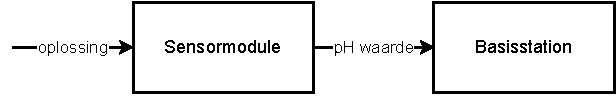
\includegraphics[width=\textwidth]{toplevelDiagram}
    \end{figure}

\end{frame}

\begin{frame}
    \frametitle{Sensormodule}

    \begin{figure}
        \centering
        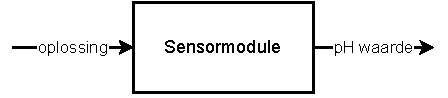
\includegraphics[width=\textwidth]{topLevelModuleOnly}
    \end{figure}

\end{frame}

%\subsection*{Eisen}
\begin{frame}
    \frametitle{Systeem eisen}

    \begin{table}[ht]
        \centering
        \begin{tabular}{|l|c c|l|}
            \hline
            Beschrijving                 & Min               & Max   & Eenheid           \\
            \hline 
            Afwijking                    &                   & 0.05  & pH                \\ 
            Bereik                       & 2                 & 10    & pH                \\
            Bandbreedte                  & 10                &       & Hz                \\
            $\mathrm{SNR}_{uit}$         & 36                &       & \qty{}{\decibel}  \\
            Rf afstand                   &                   & 10    & \qty{}{\meter}    \\
            Rf BER                       & $1\times10^{-5}$  &       &                   \\
            Levensduur                   & 48                &       & \qty{}{\hour}     \\
            Gemiddeld gebruikte vermogen &                   & 10    & mW                \\
            Energy harvesting            & $>$ 0             &       & mW                \\
            \hline
        \end{tabular}
        \caption{Systeemspecificaties.}
        \label{tab:systemSpecs}
    \end{table}

\end{frame}

\begin{frame}
    \frametitle{Systeemdiagram van de sensormodule}
    
    \begin{figure}
        \centering
        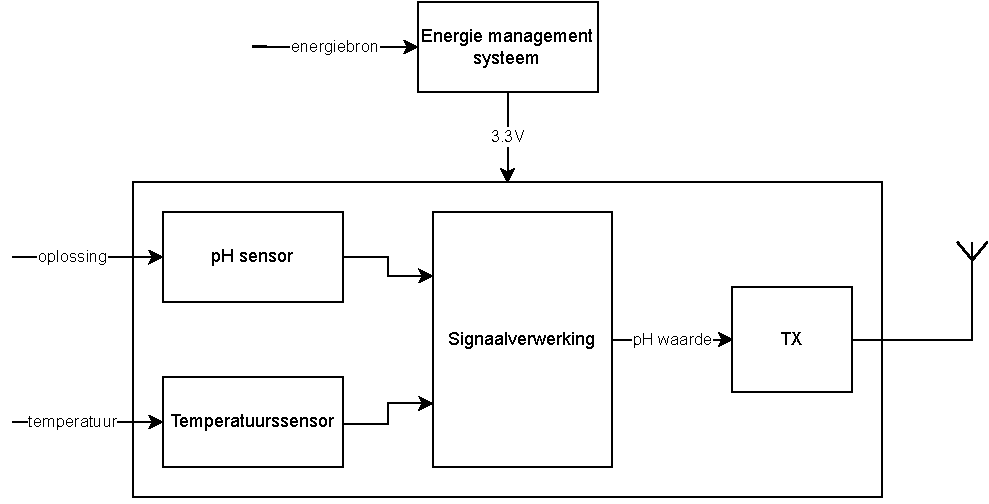
\includegraphics[width=\textwidth]{moduleDiagram.pdf}
    \end{figure}
    
\end{frame}
\begin{frame}
    \frametitle{Signaalverwerking}
    
    \begin{figure}
        \centering
        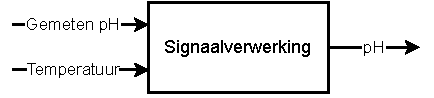
\includegraphics[width=\textwidth]{signaalverwerkingBlokje}
    \end{figure}

\end{frame}

\begin{frame}
    \frametitle{Signaalverwerking}
    
    \begin{figure}
        \centering
        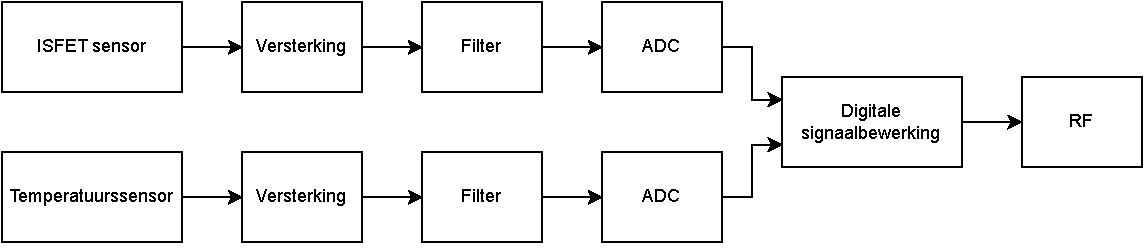
\includegraphics[width=\textwidth]{analogeBewerkingsFunctie}
    \end{figure}

\end{frame}

\begin{frame}
    \frametitle{Energie budget}
    \begin{table}[ht]
        \centering
        \begin{tabular}{l|l}
            Func. blok          & Vermogen [mW] \\
            \hline                              
            Reken $U_{GS}\rightarrow$pH & 0.6   \\
            ADC                 & 1             \\
            AA-filter           & 0.2           \\
            Meet $U_{GS}$       & 0.2           \\
            Zenden              & 5             \\
            Oplader             & 0.5           \\
            Beveiliging         & 0.5           \\
            Spanningsregeling   & 1             \\ 
            \hline
            \hline
            Totaal              & 9
            
        \end{tabular}
        \label{tab:energieBudgetEstimatie}
    \end{table}
    
\end{frame}
\begin{frame}
    \frametitle{Uitleesschakeling}
    
    \only<1>{
        \begin{figure}
            \centering
            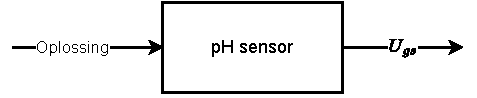
\includegraphics[width=\textwidth]{pHBlokje}
        \end{figure}
    }

    \only<2>{
        \begin{figure}
            \centering
            \def\svgwidth{0.6\textwidth}
            \input{ISFETCircuitBest.pdf_tex}
        \end{figure}
    }

\end{frame}

\begin{frame}
    \frametitle{Energie}

    \begin{wrapfigure}{r}{0.5\textwidth}
        \centering
        \def\svgwidth{0.5\textwidth}
        \input{ISFETCircuitBest.pdf_tex}
    \end{wrapfigure}
    
    $P_{statisch} = P_{n,quiescent} + U_{dd}I_{ds}$
    \pause
    \vspace{1cm}

    $U_{dd}=3v3$

    $I_{ds}=50\mu$
    \pause

    $P_{statisch} = P_{n,quiescent} + 165\mu\mathrm{W}$
\end{frame}
\subsection{ADC}

% min bits
Een ADC zet analoge signaal om in digitale signalen. Hierbij heeft een ADC een zekere resolutie. Deze resolutie is afhankelijk van het aantal bits dat de ADC heeft. Een andere oorzaak van fouten die bij een ADC kunnen optreden is de sample frequentie. Als deze niet hoog genoeg is zal dit ook een fout creëren.

\subsubsection{Number of bits} \label{sec:ADC:numBits}
De resolutie van een ADC kan worden uitgerekend met \cref{eq:adcRes}, waarbij n het aantal bits van de ADC is.
\begin{equation}\label{eq:adcRes}
    Q=\frac{1}{2^n-1}
\end{equation}

Met \cref{eq:meanSquareErrorADC} is de fout die ontstaat door de eindige resolutie van de ADC te berekenen \cite{MJHcalcADC}. In het geval er uit specificaties een maximale $\overline{e_{eff}^2}$ kan worden gehaald kan met \cref{eq:calcNeededQ} de minimale resolutie worden berekend.
\begin{equation}\label{eq:meanSquareErrorADC} 
    \overline{e_{eff}^2}=\frac{Q^2}{12}
\end{equation}
\begin{equation}\label{eq:calcNeededQ}
    Q=\sqrt{12\cdot\overline{e_{eff}^2}}
\end{equation}

% $\overline{e_{eff}^2}$ mag niet groter dan de helft van het ingangsruis vermogen zijn (noise figure van 1.5dB).
Voor dit ontwerp is er een noise figure gegeven en is de SNR voor het kleinste signaal bekend. Ook is het kleinste ingangssignaal bekend. Door gebruik te maken van \cref{eq:calcSpecifiedRmsError}, is het mogelijk om uit te rekenen hoe groot de fout ten gevolge van de eindige resolutie van de ADC mag zijn.
\begin{equation}\label{eq:calcSpecifiedRmsError}
    \overline{e_{eff}^2}=\left(10^{\frac{NF}{10}}-1\right)\left(\frac{S_{rms}}{10^{SNR+NF/20}}\right)^2
\end{equation}

Door gebruik te maken van \cref{eq:adcRes,eq:meanSquareErrorADC,eq:calcSpecifiedRmsError}, kan het minimum aantal bits van de benodigde ADC berekend worden met \cref{eq:calcMinNumberADCbits}.
\begin{equation}\label{eq:calcMinNumberADCbits}
    n=\left\lceil\log_2\left(\frac{1}{Q}+1\right)\right\rceil
\end{equation}

\subsubsection{Sample frequentie}\label{sec:ADC:sampleFreq}
% min sample rate
De maximale sample rate voor een gegeven ADC is afhankelijk van het aantal bits van de ADC en de hoogste te meten signaal frequentie. De hoogste sample rate zal dan ook geen fouten meer introduceren \cite{MJHcalcADC}. De formule om de hoogste sample rate mee te berekenen is gegeven door \cref{eq:ADCmaxFs}.
\begin{equation}\label{eq:ADCmaxFs}
    f_{s,max}\left(n\right)=2^n\pi f_h
\end{equation}
In veel gevallen is de hoogste sample rate niet van interesse omdat die zo hoog ligt dat het een puur theoretisch getal is. Om een minimale sample frequentie te berekenen moet er eerst een toe te stane fout bepaald worden. Deze fout kan door middel van een noise figure gespecificeerd worden. Met een bekende noise figure kan door gebruik te maken van \cref{eq:ADCmaxSampleError} is er een factor uit te rekenen die gebruikt kan worden in \cref{eq:ADCminFs} om de minimale sample frequentie uit te rekenen.
\begin{equation}\label{eq:ADCmaxSampleError}
    E=10^{\frac{-NF}{10}}
\end{equation}
\begin{equation}\label{eq:ADCminFs}
    f_{s,min}\left(E\right)=\frac{\pi f_h}{E}
\end{equation}
\subsection{Filter}
Tussen de ADC en de uitleesschakeling van de sensor zit een filter. Dit filter zorgt ervoor dat alle frequenties buiten de bandbreedte weggefilterd worden. Er is gekozen om hiervoor een eerste orde filter te gebruiken.
De schakeling van dit filter is te zien in \autoref{fig:filterCircuit}. De kantelfrequentie het filter ligt aan de waardes van $C$ en $R$, volgens \autoref{eq:cutoffFreq}.

\subsubsection{Ruis}
De spectrale ruisdichtheid aan de ingang van het filter is te berekenen met \autoref{eq:filterNoiseDensity}.
De spectrale ruisdichtheid aan de uitgang van het filter is hetzelfde als die van de spanningsdeler in \autoref{sec:referenceVoltage}. Deze is te berekenen met \autoref{eq:dividerNoise}.

\begin{figure}[ht]
    \centering
    \def\svgwidth{0.3\textwidth}
    \subsection{Filter}
Tussen de ADC en de uitleesschakeling van de sensor zit een filter. Dit filter zorgt ervoor dat alle frequenties buiten de bandbreedte weggefilterd worden. Er is gekozen om hiervoor een eerste orde filter te gebruiken.
De schakeling van dit filter is te zien in \autoref{fig:filterCircuit}. De kantelfrequentie het filter ligt aan de waardes van $C$ en $R$, volgens \autoref{eq:cutoffFreq}.

\subsubsection{Ruis}
De spectrale ruisdichtheid aan de ingang van het filter is te berekenen met \autoref{eq:filterNoiseDensity}.
De spectrale ruisdichtheid aan de uitgang van het filter is hetzelfde als die van de spanningsdeler in \autoref{sec:referenceVoltage}. Deze is te berekenen met \autoref{eq:dividerNoise}.

\begin{figure}[ht]
    \centering
    \def\svgwidth{0.3\textwidth}
    \subsection{Filter}
Tussen de ADC en de uitleesschakeling van de sensor zit een filter. Dit filter zorgt ervoor dat alle frequenties buiten de bandbreedte weggefilterd worden. Er is gekozen om hiervoor een eerste orde filter te gebruiken.
De schakeling van dit filter is te zien in \autoref{fig:filterCircuit}. De kantelfrequentie het filter ligt aan de waardes van $C$ en $R$, volgens \autoref{eq:cutoffFreq}.

\subsubsection{Ruis}
De spectrale ruisdichtheid aan de ingang van het filter is te berekenen met \autoref{eq:filterNoiseDensity}.
De spectrale ruisdichtheid aan de uitgang van het filter is hetzelfde als die van de spanningsdeler in \autoref{sec:referenceVoltage}. Deze is te berekenen met \autoref{eq:dividerNoise}.

\begin{figure}[ht]
    \centering
    \def\svgwidth{0.3\textwidth}
    \input{img/filter.pdf_tex}
    \caption{Het eerste-orde filter.}
    \label{fig:filterCircuit}
\end{figure}

% TODO: BEPAAL OVERDRACHT

\begin{equation} \label{eq:cutoffFreq}
    2\pi f_c = \omega_c = \frac{1}{RC}
    \tagaddtext{[\si{\radian\per\second}]}
\end{equation}

% \begin{equation} \label{eq:filterTransfer}
%     H(s) = \frac{1}{1+sRC}
% \end{equation}

\begin{equation} \label{eq:filterNoiseDensity}
    S_{u_{in}} = 4kTR
    \tagaddtext{[\si{\volt\squared\per\hertz}]}
\end{equation}

% De signaal-ruis verhouding aan de uitgang van dit filter is te berekenen met \autoref{eq:filterSNR}
% \begin{equation}\label{eq:filterSNR}
%     \mathrm{SNR} = 20\log\left(U_{out,min}\sqrt{\frac{C}{kT}}\right)
%     \tagaddtext{[\si{\decibel}]}
% \end{equation}

\subsubsection{Vermogen}
Het vermogensverbruik van het filter is te berekenen met \autoref{eq:filterPowerLaplace}.
\begin{equation} \label{eq:filterPowerLaplace}
    P = \frac{U_{in,max}^2}{\left|R + \frac{1}{sC}\right|}
    \tagaddtext{[\si{\watt}]}
\end{equation}
Omdat volgens \autoref{eq:cutoffFreq} $R$ te definiëren is in $\omega_c$ en $C$, volgt hieruit \autoref{eq:filterPower}.
\begin{equation} \label{eq:filterPower}
    P = \frac{1}{\sqrt{2}}\omega_cCU_{in,max}^2
    \tagaddtext{[\si{\watt}]}
\end{equation}
Uit deze formule is te zien dat het vermogensverbruik lineair evenredig is met de condensatorwaarde. Om het vermogensverbruik te minimaliseren moet dus een zo klein mogelijk condensatorwaarde gekozen worden. Aangezien de noise-figure van dit filter maximaal 3dB mag zijn, mag dit filter maximaal evenveel spanningsruis genereren als het systeem ervoor. Hieruit volgt \autoref{eq:dividerNoise}, waarmee de minimale condensatorwaarde te berekenen is. Hierbij is $u_{n,in}$ de ruisspanning aan de ingang van het filter.
\begin{equation} \label{eq:filterCapMin}
    C_{min} = \frac{kT}{u_{n,in}^2}
    \tagaddtext{[\si{\farad}]}
\end{equation}
    \caption{Het eerste-orde filter.}
    \label{fig:filterCircuit}
\end{figure}

% TODO: BEPAAL OVERDRACHT

\begin{equation} \label{eq:cutoffFreq}
    2\pi f_c = \omega_c = \frac{1}{RC}
    \tagaddtext{[\si{\radian\per\second}]}
\end{equation}

% \begin{equation} \label{eq:filterTransfer}
%     H(s) = \frac{1}{1+sRC}
% \end{equation}

\begin{equation} \label{eq:filterNoiseDensity}
    S_{u_{in}} = 4kTR
    \tagaddtext{[\si{\volt\squared\per\hertz}]}
\end{equation}

% De signaal-ruis verhouding aan de uitgang van dit filter is te berekenen met \autoref{eq:filterSNR}
% \begin{equation}\label{eq:filterSNR}
%     \mathrm{SNR} = 20\log\left(U_{out,min}\sqrt{\frac{C}{kT}}\right)
%     \tagaddtext{[\si{\decibel}]}
% \end{equation}

\subsubsection{Vermogen}
Het vermogensverbruik van het filter is te berekenen met \autoref{eq:filterPowerLaplace}.
\begin{equation} \label{eq:filterPowerLaplace}
    P = \frac{U_{in,max}^2}{\left|R + \frac{1}{sC}\right|}
    \tagaddtext{[\si{\watt}]}
\end{equation}
Omdat volgens \autoref{eq:cutoffFreq} $R$ te definiëren is in $\omega_c$ en $C$, volgt hieruit \autoref{eq:filterPower}.
\begin{equation} \label{eq:filterPower}
    P = \frac{1}{\sqrt{2}}\omega_cCU_{in,max}^2
    \tagaddtext{[\si{\watt}]}
\end{equation}
Uit deze formule is te zien dat het vermogensverbruik lineair evenredig is met de condensatorwaarde. Om het vermogensverbruik te minimaliseren moet dus een zo klein mogelijk condensatorwaarde gekozen worden. Aangezien de noise-figure van dit filter maximaal 3dB mag zijn, mag dit filter maximaal evenveel spanningsruis genereren als het systeem ervoor. Hieruit volgt \autoref{eq:dividerNoise}, waarmee de minimale condensatorwaarde te berekenen is. Hierbij is $u_{n,in}$ de ruisspanning aan de ingang van het filter.
\begin{equation} \label{eq:filterCapMin}
    C_{min} = \frac{kT}{u_{n,in}^2}
    \tagaddtext{[\si{\farad}]}
\end{equation}
    \caption{Het eerste-orde filter.}
    \label{fig:filterCircuit}
\end{figure}

% TODO: BEPAAL OVERDRACHT

\begin{equation} \label{eq:cutoffFreq}
    2\pi f_c = \omega_c = \frac{1}{RC}
    \tagaddtext{[\si{\radian\per\second}]}
\end{equation}

% \begin{equation} \label{eq:filterTransfer}
%     H(s) = \frac{1}{1+sRC}
% \end{equation}

\begin{equation} \label{eq:filterNoiseDensity}
    S_{u_{in}} = 4kTR
    \tagaddtext{[\si{\volt\squared\per\hertz}]}
\end{equation}

% De signaal-ruis verhouding aan de uitgang van dit filter is te berekenen met \autoref{eq:filterSNR}
% \begin{equation}\label{eq:filterSNR}
%     \mathrm{SNR} = 20\log\left(U_{out,min}\sqrt{\frac{C}{kT}}\right)
%     \tagaddtext{[\si{\decibel}]}
% \end{equation}

\subsubsection{Vermogen}
Het vermogensverbruik van het filter is te berekenen met \autoref{eq:filterPowerLaplace}.
\begin{equation} \label{eq:filterPowerLaplace}
    P = \frac{U_{in,max}^2}{\left|R + \frac{1}{sC}\right|}
    \tagaddtext{[\si{\watt}]}
\end{equation}
Omdat volgens \autoref{eq:cutoffFreq} $R$ te definiëren is in $\omega_c$ en $C$, volgt hieruit \autoref{eq:filterPower}.
\begin{equation} \label{eq:filterPower}
    P = \frac{1}{\sqrt{2}}\omega_cCU_{in,max}^2
    \tagaddtext{[\si{\watt}]}
\end{equation}
Uit deze formule is te zien dat het vermogensverbruik lineair evenredig is met de condensatorwaarde. Om het vermogensverbruik te minimaliseren moet dus een zo klein mogelijk condensatorwaarde gekozen worden. Aangezien de noise-figure van dit filter maximaal 3dB mag zijn, mag dit filter maximaal evenveel spanningsruis genereren als het systeem ervoor. Hieruit volgt \autoref{eq:dividerNoise}, waarmee de minimale condensatorwaarde te berekenen is. Hierbij is $u_{n,in}$ de ruisspanning aan de ingang van het filter.
\begin{equation} \label{eq:filterCapMin}
    C_{min} = \frac{kT}{u_{n,in}^2}
    \tagaddtext{[\si{\farad}]}
\end{equation}

\begin{frame}
    \frametitle{Rf}

    \begin{figure}
        \centering
        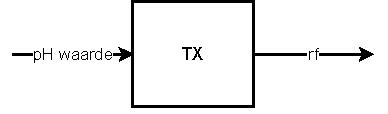
\includegraphics[width=0.9\textwidth]{rfBlock}
    \end{figure}

\end{frame}


\begin{frame}
    \frametitle{Ontvangstgevoeligheid}

    \begin{table}
        \centering
        \begin{tabular}{l|c}
            Eigenschap & Waarde \\\hline
            BER & $1\times10^{-5}$ \\
            $\Delta N$ & -105 dBm \\
            Noise Figure & 12.6 dB \\
            Modulatie & GFSK \\
        \end{tabular}
        \caption{Eigenschappen van de ontvanger op het basisstation.}
    \end{table}

    \pause 

    $S_{or}=-57$ dBm bij B = \qty{1}{\mega\hertz}

    $S_{or}=-54$ dBm bij B = \qty{2}{\mega\hertz}

\end{frame}

\begin{frame}
    \frametitle{Minimum zendvermogen}

    \begin{table}
        \centering
        \begin{tabular}{l|c}
            Eigenschap & Waarde \\\hline
            Afstand & \qty{10}{\meter} \\
            Hoogte & \qty{1}{\meter} \\
        \end{tabular}
        \caption{Antenne plaatsing.}
    \end{table}

    Path loss = 53.2 dB

    \pause

    $\Rightarrow$

    $P_{z}=-4$dBm bij B = \qty{1}{\mega\hertz}

    $P_{z}=-1$dBm bij B = \qty{2}{\mega\hertz}
\end{frame}

\begin{frame}
    \frametitle{Energie en gemiddeld vermogen}

    Energie kosten per verzonden pakket:
    \begin{equation*}
        E_{z,p}=\frac{l}{DR}P_z
    \end{equation*}

    \pause

    $E_{z,p}=$\qty{117.8}{\nano\joule} bij B = \qty{1}{\mega\hertz}

    $E_{z,p}=$\qty{117.6}{\nano\joule} bij B = \qty{2}{\mega\hertz}

    \pause

    \vspace{1cm}
    $\overline{P_z}=E_{z,p}f_s$ $\Rightarrow$ \qty{7.1}{\micro\watt} in geval van een bandbreedte van \qty{2}{\mega\hertz}

\end{frame}
% # Ontwerp
% ## ...
% ##


\subsection{De oplaadbare voeding van het systeem} \label{sec:energy}

De sensormodule heeft energie nodig om te functioneren. Deze energie moet geleverd worden door een energie management systeem in de vorm van een constante spanning. Het voedingsblok ligt buiten het signaalverwerkingspad, zoals te zien is in \cref{fig:moduleDiagram_energie}.

\begin{figure}[!htb]
    \centering
    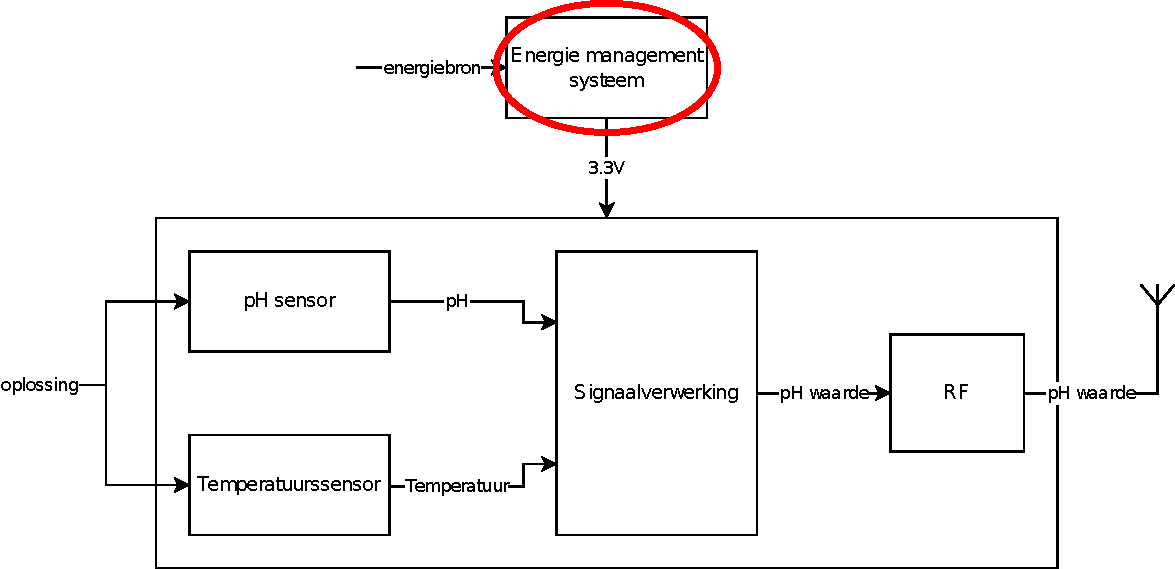
\includegraphics[width=.7\textwidth]{moduleDiagram_energie}
    \caption{De locatie van het energie management systeem in het blokschema van de sensormodule.}
    \label{fig:moduleDiagram_energie}
\end{figure}

Het energie management systeem moet energie kunnen opnemen uit de omgeving, en dit kunnen opslaan. Hiervoor zijn een energy harvesting systeem en een accu nodig.

\subsubsection{Energy Harvesting} \label{sec:harvesting}

Vanuit de opdrachtdefinitie is er gekozen voor een piëzo-element. Deze piëzo kan mechanische trillingen omzetten naar elektrische energie. Deze energie kan gebruikt worden om de accu op te laden of het energieverbruik van de module te verminderen.

Een piëzo-element produceert energie in de vorm van wisselspanning. Deze spanningen kunnen oplopen tot spanningen boven de \qty{20}{\volt}.% TODO: bron????
Hierdoor zal er, naast een gelijkrichter en een spanningsregelaar, ook een beveiliging tussen het piëzo-element en de rest van het systeem geplaatst moeten worden.


\subsubsection{Accu} \label{sec:batterijOntwerp}
Er zijn veel verschillende soorten soorten oplaadbare batterijen die gebruikt kunnen worden bij een sensor module.
Voor de type sensor module waar dit verslag over gaat is gekeken naar 4 verschillende oplaadbare accu opties\cite{battery-comparison}:

\begin{enumerate}
    \item Lithium-Ion (Li-Ion)
    \item Lithium Polymeer (Li-Po)
    \item Zebra (Zout nickel)
    \item Nickel-Cadmium (Ni-Cd)
\end{enumerate}

In onderzoek \cite{battery-comparison} is het duidelijk aangetoond dat Li-Po het hoogste energiedichtheid heeft. Dit zou een praktische overweging zijn om de sensor module compact te houden. Dit heeft ervoor gezorgd dat voor de sensor module ontwerp een LiPo gekozen is als batterij. Spanning van een cel (1s) LiPo is maximaal \qty{4.2}{\volt} en minimaal veilige spanning is \qty{2.7}{\volt}\cite{BatteryComparison}. Dit is een van de specificaties van de batterij management systeem.


\subsubsection{Voeding} \label{sec:voeding}
De voedingsspanning is gekozen vanuit de maximale spanning die nodig is voor de ISFET sensor\cite{isfet}. Hieruit volgt een maximale systeemspanning van \qty{3.3}{\volt}.

Zoals te lezen in \cref{sec:batterijOntwerp} is er gekozen voor LiPo batterij technologie. De batterij heeft een beveiliging voor beide op- en ontladen nodig. De celspanning moet omgezet worden naar systeemspanning van \qty{3.3}{\volt}. Dit kan op meerdere manieren gedaan worden. Twee hiervan zijn een DC-DC buck-boost converter en een low dropout regelaar (LDO). De buck-boost converter is efficiënter dan de LDO, maar heeft een minder stabiele uitgang. Hierdoor is ervoor gekozen om beide soorten regelaar te gebruiken. Dit is te zien in \cref{fig:voedingSchematisch}. Het digitale gedeelte van het systeem wordt gevoed door een buck-boost converter; de spanningsrimpel van de buck-boost converter maakt minder uit voor een goed ontkoppelde microcontroller.
De uitgang van de buck-boost converter wordt vervolgens gestabiliseerd door een LDO, die het analoge gedeelte van het systeem voedt. De uitgangsspanning van de LDO zal iets lager zijn dan de uitgang van de buck-boost converter, wat geen problemen zal vormen zolang het verschil minimaal is.

Zoals beschreven in \cref{sec:harvesting} moet de uitgang van het piëzo-element gelijk gericht en beschermt worden. In \cref{fig:voedingSchematisch} wordt het gelijkrichten gedaan door de AC-DC omvormer.

Voor energy harvesting is er een piëzo-element gekozen. Een piëzo-element kan gezien worden als een AC bron. Deze AC bron moet omgezet worden naar DC die door het systeem gebruikt kan worden om de batterij mee op te laden. De AC bron wordt met een gelijkrichter naar DC omgezet. Deze DC spanning is niet hetzelfde als de systeemspanning dus die moet omgezet worden naar een spanning die de batterij in gaat, zodat de batterij kan opladen.

\begin{figure}[!htb]
    \centering
    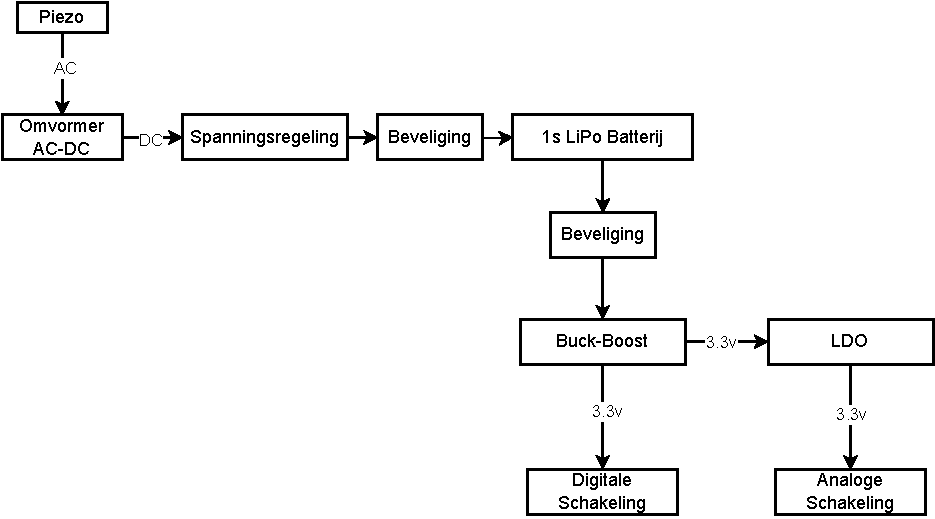
\includegraphics{voedingSchematisch.pdf}
    \caption{Voeding schematisch}
    \label{fig:voedingSchematisch}
\end{figure}



\subsubsection{Energie budget}\label{sec:energyBudgets}
Voor het energiebudget zijn de waardes in \cref{tab:energieBudgetEstimatie} gekozen. Elk van deze waardes ligt boven het theoretisch berekende minimum van het respectievelijke systeemonderdeel. De som van de vermogens is \qty{9}{\milli\watt}, wat onder het maximale toegestane energieverbruik van \qty{10}{\milli\watt} ligt.


\begin{table}[!htb]
    \centering
    \begin{tabular}{l|l}
        Func. blok          & Vermogen [mW] \\
        \hline
        Reken $U_{GS}\rightarrow$pH & 0.6   \\
        ADC                 & 1             \\
        AA-filter           & 0.2           \\
        Meet $U_{GS}$       & 0.2           \\
        Zenden              & 5             \\
        Oplader             & 0.5           \\
        Beveiliging         & 0.5           \\
        Spanningsregeling   & 1             \\
        \hline
        \hline
        Totaal              & 9

    \end{tabular}
    \caption{Energie budget}
    \label{tab:energieBudgetEstimatie}
\end{table}




% \section{Sensor data naar pH omzetten}

\subsection*{Uitlezen ISFET}

    \begin{frame}
        \frametitle{Principe schakeling}
    
        \begin{figure}
            \centering
            \def\svgwidth{0.6\textwidth}
            \input{ISFETCircuitBest.pdf_tex}
        \end{figure}
    
    \end{frame}
    \begin{frame}
        \frametitle{Ruis analyse}
    
        \begin{figure}
            \centering
            \def\svgwidth{0.6\textwidth}
            \input{ISFETCircuitBestNoise.pdf_tex}
        \end{figure}
        \begin{equation}\label{eq:measureNoiseOut}
            S_{u_{{n,out}}} = \left(S_{u_{{n,ref}}} + S_{u_{{n,n}}} + S_{i_{{n,in}}}\left(Z_{fet} // R\right)^2\right) \cdot H^2(\ph)
        \end{equation}
    
    \end{frame}
    \begin{frame}
        \frametitle{Energie}

        $U_{dd}=3v3$

        \noindent
        $I_{ds}=50\mu$A
    
        \begin{equation}\label{eq:measurePower}
            P_{statisch} = P_{n,quiescent} + U_{dd}I_{ds}
        \end{equation}

        \pause

        \begin{equation}
            P_{statisch} = P_{n,quiescent} + 165\mu\mathrm{W}
        \end{equation}
    
    \end{frame}

    \subsection*{ADC}
    \begin{frame}
        \frametitle{Eisen}
    
        \begin{table}[ht]
    \centering
    \begin{tabular}{l|c|l}
        Symbol      & Waarde & Eenheid\\\hline
        $SNR_{in}$  & 37        & dB\\
        NF          & 3         & dB\\
        $u_{in}$    & 2.5       & mV\\
    \end{tabular}
    \caption{De eisen voor het omzetten van het analoge signaal naar een digitaal signaal.}
    \label{tab:systemSpecADC}
\end{table}
    
    \end{frame}
    \begin{frame}
        \frametitle{Minimum aantal bits}
        \centering

        De toelaatbare fout ten gevolge van de eindige resolutie van de ADC
        \begin{equation}\label{eq:calcSpecifiedRmsError}
            \overline{e_{eff}^2}=\left(10^{\frac{NF}{10}}-1\right)\left(\frac{S_{rms}}{10^{\left(SNR+NF\right)/20}}\right)^2
        \end{equation}
        \pause

        Berekenen minimum benodigde ADC resolutie
        \begin{equation}\label{eq:calcNeededQ}
            Q=\sqrt{12\cdot\overline{e_{eff}^2}}
        \end{equation}
        \pause

        Berekenen minimum aantal bits van de ADC op basis van de minimaal benodigde ADC resolutie 
        \begin{equation}\label{eq:calcMinNumberADCbits}
            n=\left\lceil\log_2\left(\frac{1}{Q}+1\right)\right\rceil=14
        \end{equation}
    
    \end{frame}

    \begin{frame}
        \frametitle{Sample frequentie}
        \centering
        
        Toelaatbare fout
        \begin{equation}\label{eq:ADCmaxSampleError}
            E=10^{\frac{-NF}{10}}
        \end{equation}
        \pause

        Minimale sample frequentie berekenen
        \begin{equation}\label{eq:ADCminFs}
            f_{s,min}=\frac{\pi f_h}{E}=45
        \end{equation}
    
    \end{frame}

    \subsection*{AA filter}
    \begin{frame}
        \frametitle{Eisen anti aliasing filter}
        
        \centering

        Dempen 22.5Hz


        $P_{max}=200\mu$W


        $NF=3\si{\decibel}$

        %TODO! Voeg hier een afbeelding van een RC filter
        [Voeg hier een afbeelding van een RC filter]
    
    \end{frame}
    \begin{frame}
        \frametitle{Ruis \& vermogensanalyse RC filter}
    
        \begin{equation}\label{eq:dividerNoise}
            u_{n,out}^2 = \frac{kT}{C}
        \end{equation}

        \begin{equation} \label{eq:filterPower}
            P = \frac{1}{\sqrt{2}}\omega_cCU_{in,max}^2
        \end{equation}

        \pause

        \begin{equation} \label{eq:filterCapMin}
            C_{min} = \frac{kT}{u_{n,in}^2}
        \end{equation}

        \begin{equation}
            R = \frac{1}{2\pi fC}
        \end{equation}
    
    \end{frame}
    \begin{frame}
        \frametitle{AA filter}
    
        \begin{table}[ht]
            \centering
            \begin{tabular}{l|l|l}
                Symbool & Waarde & Eenheid \\
                \hline
                $C$         & 82    & $\si{\nano\farad}$\\
                $R$         & 180   & $\si{\kilo\ohm}$  \\
                $f_c$       & 10.8  & $\si{\hertz}$     \\
                $P$         & 408   & $\si{\nano\watt}$ \\
                $u_{n,out}$ & 225   & $\si{\nano\volt}$ \\
                NF          & 0.23  & $\si{\decibel}$   \\
            \end{tabular}
            \caption{De gekozen waardes van het filter, en de resulterende vermogens- en ruiseigenschappen.}
            \label{tab:filterValues}
        \end{table}
    
    \end{frame}
    \begin{frame}
        \frametitle{Effecten van de load}
    
        Spanningsdeler met de ADC, hierdoor wordt het ingangssignaal kleiner.
    
    \end{frame}

    \subsection*{Berekenen pH}
    \begin{frame}
        \frametitle{Gemeten waarde omrekenen naar pH}
        
        %TODO jochem doe werk/voeg dingen toe
        % $\mathrm{CAL_{\mathrm{pH,H}}}=7$

        % $\mathrm{CAL_{\mathrm{pH,L}}}=4$

        % \begin{equation}
        %     \mathrm{pH}=\frac{\mathrm{S}-\mathrm{CAL_{\mathrm{ADC,L}}}}{\mathrm{CAL_{\mathrm{ADC,H}}}-\mathrm{CAL_{\mathrm{ADC,L}}}}\left(\mathrm{CAL_{\mathrm{pH,H}}}-\mathrm{CAL_{\mathrm{pH,L}}}\right)+\mathrm{CAL_{\mathrm{pH,L}}}
        % \end{equation}
    
    \end{frame}
% % # Ontwerp
% ## ...
% ##


\subsection{De oplaadbare voeding van het systeem} \label{sec:energy}

De sensormodule heeft energie nodig om te functioneren. Deze energie moet geleverd worden door een energie management systeem in de vorm van een constante spanning. Het voedingsblok ligt buiten het signaalverwerkingspad, zoals te zien is in \cref{fig:moduleDiagram_energie}.

\begin{figure}[!htb]
    \centering
    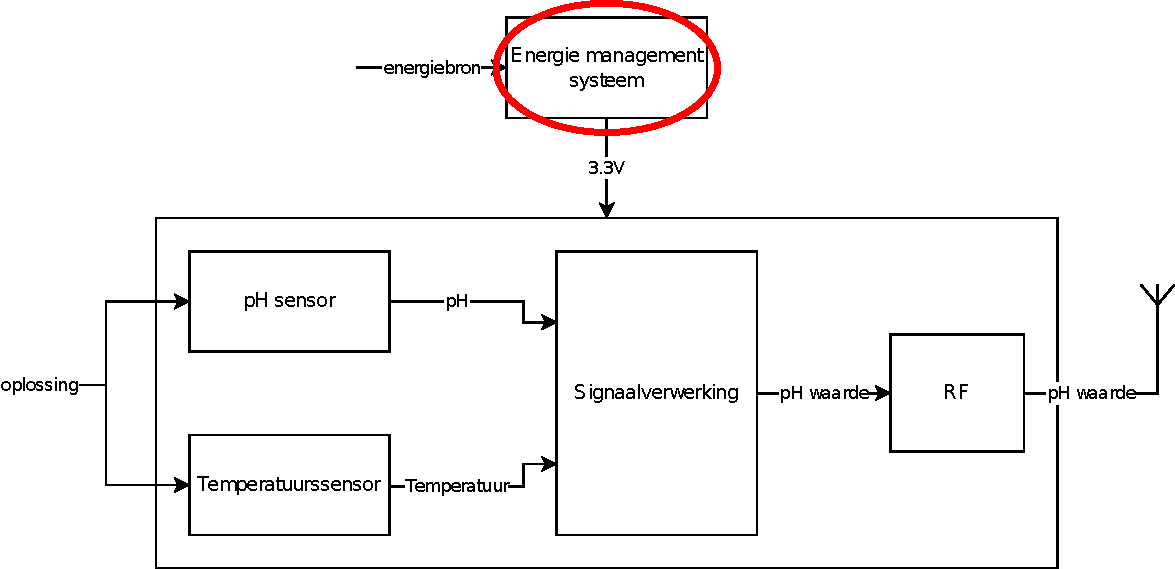
\includegraphics[width=.7\textwidth]{moduleDiagram_energie}
    \caption{De locatie van het energie management systeem in het blokschema van de sensormodule.}
    \label{fig:moduleDiagram_energie}
\end{figure}

Het energie management systeem moet energie kunnen opnemen uit de omgeving, en dit kunnen opslaan. Hiervoor zijn een energy harvesting systeem en een accu nodig.

\subsubsection{Energy Harvesting} \label{sec:harvesting}

Vanuit de opdrachtdefinitie is er gekozen voor een piëzo-element. Deze piëzo kan mechanische trillingen omzetten naar elektrische energie. Deze energie kan gebruikt worden om de accu op te laden of het energieverbruik van de module te verminderen.

Een piëzo-element produceert energie in de vorm van wisselspanning. Deze spanningen kunnen oplopen tot spanningen boven de \qty{20}{\volt}.% TODO: bron????
Hierdoor zal er, naast een gelijkrichter en een spanningsregelaar, ook een beveiliging tussen het piëzo-element en de rest van het systeem geplaatst moeten worden.


\subsubsection{Accu} \label{sec:batterijOntwerp}
Er zijn veel verschillende soorten soorten oplaadbare batterijen die gebruikt kunnen worden bij een sensor module.
Voor de type sensor module waar dit verslag over gaat is gekeken naar 4 verschillende oplaadbare accu opties\cite{battery-comparison}:

\begin{enumerate}
    \item Lithium-Ion (Li-Ion)
    \item Lithium Polymeer (Li-Po)
    \item Zebra (Zout nickel)
    \item Nickel-Cadmium (Ni-Cd)
\end{enumerate}

In onderzoek \cite{battery-comparison} is het duidelijk aangetoond dat Li-Po het hoogste energiedichtheid heeft. Dit zou een praktische overweging zijn om de sensor module compact te houden. Dit heeft ervoor gezorgd dat voor de sensor module ontwerp een LiPo gekozen is als batterij. Spanning van een cel (1s) LiPo is maximaal \qty{4.2}{\volt} en minimaal veilige spanning is \qty{2.7}{\volt}\cite{BatteryComparison}. Dit is een van de specificaties van de batterij management systeem.


\subsubsection{Voeding} \label{sec:voeding}
De voedingsspanning is gekozen vanuit de maximale spanning die nodig is voor de ISFET sensor\cite{isfet}. Hieruit volgt een maximale systeemspanning van \qty{3.3}{\volt}.

Zoals te lezen in \cref{sec:batterijOntwerp} is er gekozen voor LiPo batterij technologie. De batterij heeft een beveiliging voor beide op- en ontladen nodig. De celspanning moet omgezet worden naar systeemspanning van \qty{3.3}{\volt}. Dit kan op meerdere manieren gedaan worden. Twee hiervan zijn een DC-DC buck-boost converter en een low dropout regelaar (LDO). De buck-boost converter is efficiënter dan de LDO, maar heeft een minder stabiele uitgang. Hierdoor is ervoor gekozen om beide soorten regelaar te gebruiken. Dit is te zien in \cref{fig:voedingSchematisch}. Het digitale gedeelte van het systeem wordt gevoed door een buck-boost converter; de spanningsrimpel van de buck-boost converter maakt minder uit voor een goed ontkoppelde microcontroller.
De uitgang van de buck-boost converter wordt vervolgens gestabiliseerd door een LDO, die het analoge gedeelte van het systeem voedt. De uitgangsspanning van de LDO zal iets lager zijn dan de uitgang van de buck-boost converter, wat geen problemen zal vormen zolang het verschil minimaal is.

Zoals beschreven in \cref{sec:harvesting} moet de uitgang van het piëzo-element gelijk gericht en beschermt worden. In \cref{fig:voedingSchematisch} wordt het gelijkrichten gedaan door de AC-DC omvormer.

Voor energy harvesting is er een piëzo-element gekozen. Een piëzo-element kan gezien worden als een AC bron. Deze AC bron moet omgezet worden naar DC die door het systeem gebruikt kan worden om de batterij mee op te laden. De AC bron wordt met een gelijkrichter naar DC omgezet. Deze DC spanning is niet hetzelfde als de systeemspanning dus die moet omgezet worden naar een spanning die de batterij in gaat, zodat de batterij kan opladen.

\begin{figure}[!htb]
    \centering
    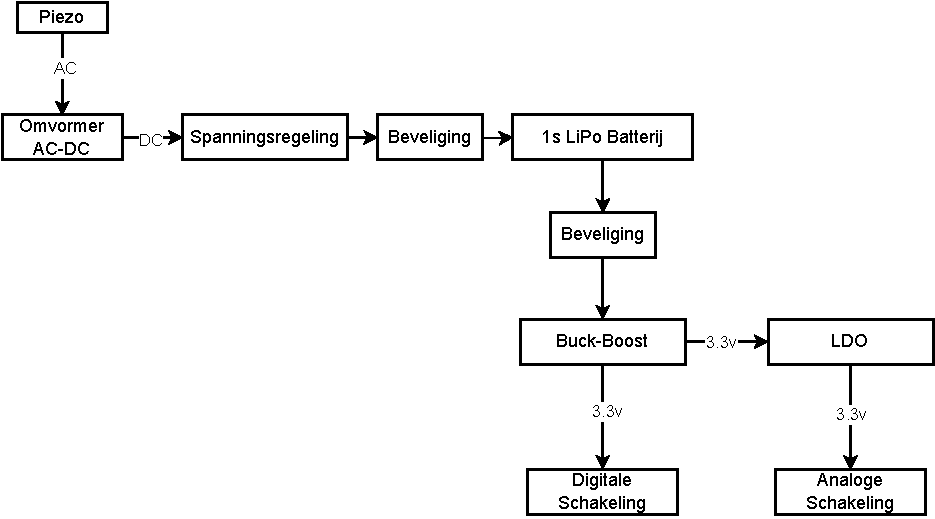
\includegraphics{voedingSchematisch.pdf}
    \caption{Voeding schematisch}
    \label{fig:voedingSchematisch}
\end{figure}



\subsubsection{Energie budget}\label{sec:energyBudgets}
Voor het energiebudget zijn de waardes in \cref{tab:energieBudgetEstimatie} gekozen. Elk van deze waardes ligt boven het theoretisch berekende minimum van het respectievelijke systeemonderdeel. De som van de vermogens is \qty{9}{\milli\watt}, wat onder het maximale toegestane energieverbruik van \qty{10}{\milli\watt} ligt.


\begin{table}[!htb]
    \centering
    \begin{tabular}{l|l}
        Func. blok          & Vermogen [mW] \\
        \hline
        Reken $U_{GS}\rightarrow$pH & 0.6   \\
        ADC                 & 1             \\
        AA-filter           & 0.2           \\
        Meet $U_{GS}$       & 0.2           \\
        Zenden              & 5             \\
        Oplader             & 0.5           \\
        Beveiliging         & 0.5           \\
        Spanningsregeling   & 1             \\
        \hline
        \hline
        Totaal              & 9

    \end{tabular}
    \caption{Energie budget}
    \label{tab:energieBudgetEstimatie}
\end{table}




% # Ontwerp
% ## ...
% ##


\subsection{De oplaadbare voeding van het systeem} \label{sec:energy}

De sensormodule heeft energie nodig om te functioneren. Deze energie moet geleverd worden door een energie management systeem in de vorm van een constante spanning. Het voedingsblok ligt buiten het signaalverwerkingspad, zoals te zien is in \cref{fig:moduleDiagram_energie}.

\begin{figure}[!htb]
    \centering
    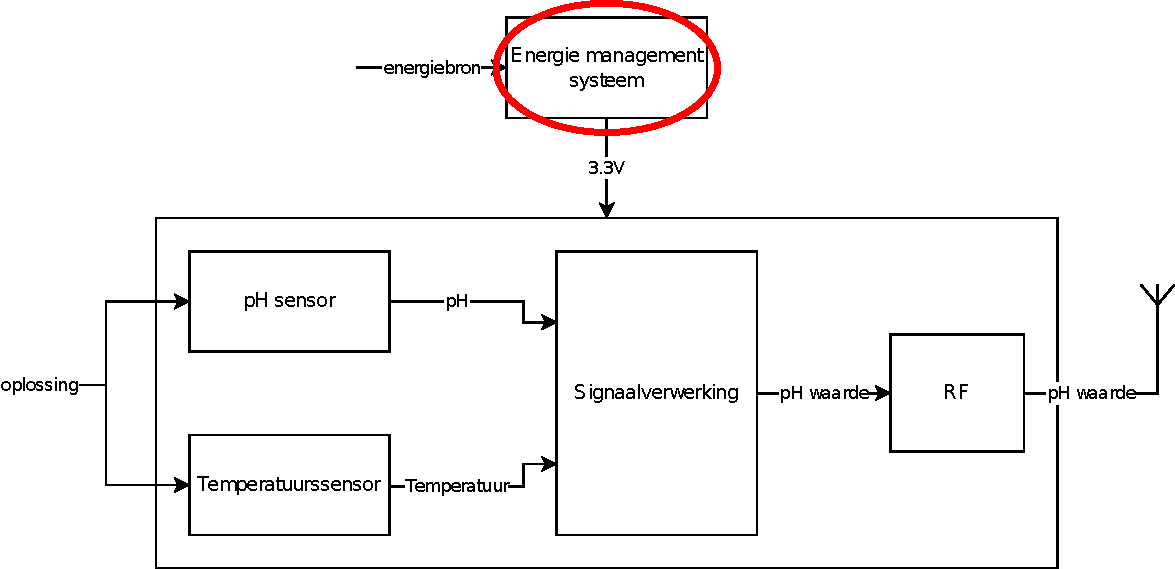
\includegraphics[width=.7\textwidth]{moduleDiagram_energie}
    \caption{De locatie van het energie management systeem in het blokschema van de sensormodule.}
    \label{fig:moduleDiagram_energie}
\end{figure}

Het energie management systeem moet energie kunnen opnemen uit de omgeving, en dit kunnen opslaan. Hiervoor zijn een energy harvesting systeem en een accu nodig.

\subsubsection{Energy Harvesting} \label{sec:harvesting}

Vanuit de opdrachtdefinitie is er gekozen voor een piëzo-element. Deze piëzo kan mechanische trillingen omzetten naar elektrische energie. Deze energie kan gebruikt worden om de accu op te laden of het energieverbruik van de module te verminderen.

Een piëzo-element produceert energie in de vorm van wisselspanning. Deze spanningen kunnen oplopen tot spanningen boven de \qty{20}{\volt}.% TODO: bron????
Hierdoor zal er, naast een gelijkrichter en een spanningsregelaar, ook een beveiliging tussen het piëzo-element en de rest van het systeem geplaatst moeten worden.


\subsubsection{Accu} \label{sec:batterijOntwerp}
Er zijn veel verschillende soorten soorten oplaadbare batterijen die gebruikt kunnen worden bij een sensor module.
Voor de type sensor module waar dit verslag over gaat is gekeken naar 4 verschillende oplaadbare accu opties\cite{battery-comparison}:

\begin{enumerate}
    \item Lithium-Ion (Li-Ion)
    \item Lithium Polymeer (Li-Po)
    \item Zebra (Zout nickel)
    \item Nickel-Cadmium (Ni-Cd)
\end{enumerate}

In onderzoek \cite{battery-comparison} is het duidelijk aangetoond dat Li-Po het hoogste energiedichtheid heeft. Dit zou een praktische overweging zijn om de sensor module compact te houden. Dit heeft ervoor gezorgd dat voor de sensor module ontwerp een LiPo gekozen is als batterij. Spanning van een cel (1s) LiPo is maximaal \qty{4.2}{\volt} en minimaal veilige spanning is \qty{2.7}{\volt}\cite{BatteryComparison}. Dit is een van de specificaties van de batterij management systeem.


\subsubsection{Voeding} \label{sec:voeding}
De voedingsspanning is gekozen vanuit de maximale spanning die nodig is voor de ISFET sensor\cite{isfet}. Hieruit volgt een maximale systeemspanning van \qty{3.3}{\volt}.

Zoals te lezen in \cref{sec:batterijOntwerp} is er gekozen voor LiPo batterij technologie. De batterij heeft een beveiliging voor beide op- en ontladen nodig. De celspanning moet omgezet worden naar systeemspanning van \qty{3.3}{\volt}. Dit kan op meerdere manieren gedaan worden. Twee hiervan zijn een DC-DC buck-boost converter en een low dropout regelaar (LDO). De buck-boost converter is efficiënter dan de LDO, maar heeft een minder stabiele uitgang. Hierdoor is ervoor gekozen om beide soorten regelaar te gebruiken. Dit is te zien in \cref{fig:voedingSchematisch}. Het digitale gedeelte van het systeem wordt gevoed door een buck-boost converter; de spanningsrimpel van de buck-boost converter maakt minder uit voor een goed ontkoppelde microcontroller.
De uitgang van de buck-boost converter wordt vervolgens gestabiliseerd door een LDO, die het analoge gedeelte van het systeem voedt. De uitgangsspanning van de LDO zal iets lager zijn dan de uitgang van de buck-boost converter, wat geen problemen zal vormen zolang het verschil minimaal is.

Zoals beschreven in \cref{sec:harvesting} moet de uitgang van het piëzo-element gelijk gericht en beschermt worden. In \cref{fig:voedingSchematisch} wordt het gelijkrichten gedaan door de AC-DC omvormer.

Voor energy harvesting is er een piëzo-element gekozen. Een piëzo-element kan gezien worden als een AC bron. Deze AC bron moet omgezet worden naar DC die door het systeem gebruikt kan worden om de batterij mee op te laden. De AC bron wordt met een gelijkrichter naar DC omgezet. Deze DC spanning is niet hetzelfde als de systeemspanning dus die moet omgezet worden naar een spanning die de batterij in gaat, zodat de batterij kan opladen.

\begin{figure}[!htb]
    \centering
    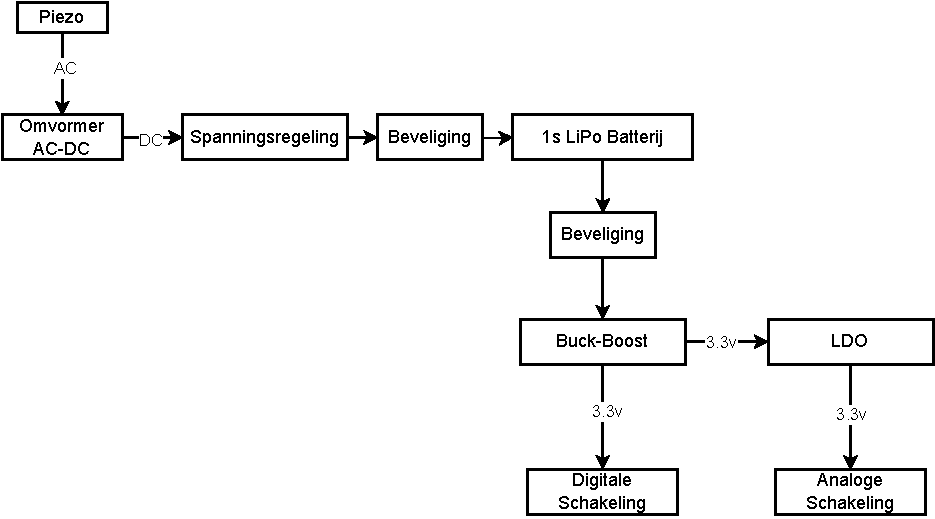
\includegraphics{voedingSchematisch.pdf}
    \caption{Voeding schematisch}
    \label{fig:voedingSchematisch}
\end{figure}



\subsubsection{Energie budget}\label{sec:energyBudgets}
Voor het energiebudget zijn de waardes in \cref{tab:energieBudgetEstimatie} gekozen. Elk van deze waardes ligt boven het theoretisch berekende minimum van het respectievelijke systeemonderdeel. De som van de vermogens is \qty{9}{\milli\watt}, wat onder het maximale toegestane energieverbruik van \qty{10}{\milli\watt} ligt.


\begin{table}[!htb]
    \centering
    \begin{tabular}{l|l}
        Func. blok          & Vermogen [mW] \\
        \hline
        Reken $U_{GS}\rightarrow$pH & 0.6   \\
        ADC                 & 1             \\
        AA-filter           & 0.2           \\
        Meet $U_{GS}$       & 0.2           \\
        Zenden              & 5             \\
        Oplader             & 0.5           \\
        Beveiliging         & 0.5           \\
        Spanningsregeling   & 1             \\
        \hline
        \hline
        Totaal              & 9

    \end{tabular}
    \caption{Energie budget}
    \label{tab:energieBudgetEstimatie}
\end{table}





\begin{frame}
    \frametitle{Rf}

    \begin{figure}
        \centering
        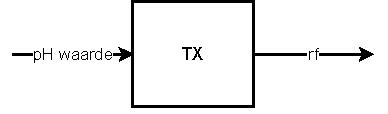
\includegraphics[width=0.9\textwidth]{rfBlock}
    \end{figure}

\end{frame}


\begin{frame}
    \frametitle{Ontvangstgevoeligheid}

    \begin{table}
        \centering
        \begin{tabular}{l|c}
            Eigenschap & Waarde \\\hline
            BER & $1\times10^{-5}$ \\
            $\Delta N$ & -105 dBm \\
            Noise Figure & 12.6 dB \\
            Modulatie & GFSK \\
        \end{tabular}
        \caption{Eigenschappen van de ontvanger op het basisstation.}
    \end{table}

    \pause 

    $S_{or}=-57$ dBm bij B = \qty{1}{\mega\hertz}

    $S_{or}=-54$ dBm bij B = \qty{2}{\mega\hertz}

\end{frame}

\begin{frame}
    \frametitle{Minimum zendvermogen}

    \begin{table}
        \centering
        \begin{tabular}{l|c}
            Eigenschap & Waarde \\\hline
            Afstand & \qty{10}{\meter} \\
            Hoogte & \qty{1}{\meter} \\
        \end{tabular}
        \caption{Antenne plaatsing.}
    \end{table}

    Path loss = 53.2 dB

    \pause

    $\Rightarrow$

    $P_{z}=-4$dBm bij B = \qty{1}{\mega\hertz}

    $P_{z}=-1$dBm bij B = \qty{2}{\mega\hertz}
\end{frame}

\begin{frame}
    \frametitle{Energie en gemiddeld vermogen}

    Energie kosten per verzonden pakket:
    \begin{equation*}
        E_{z,p}=\frac{l}{DR}P_z
    \end{equation*}

    \pause

    $E_{z,p}=$\qty{117.8}{\nano\joule} bij B = \qty{1}{\mega\hertz}

    $E_{z,p}=$\qty{117.6}{\nano\joule} bij B = \qty{2}{\mega\hertz}

    \pause

    \vspace{1cm}
    $\overline{P_z}=E_{z,p}f_s$ $\Rightarrow$ \qty{7.1}{\micro\watt} in geval van een bandbreedte van \qty{2}{\mega\hertz}

\end{frame}

% \section{Vragen}
\begin{frame}
    \frametitle{Vragen?}
    
    \centering
    Zijn er nog vragen?

\end{frame}

\end{document}